\section{Evaluation Methodology}

%\subsection{Evaluation Methodology}
Our experiments aim to answer the following three questions: (1) can our
transition matrix effectively model the noise in the training data generated
through \DS? (2) what kind of noise our approach can deal with? and (3)
whether the prior knowledge of data quality can help our approach better
handle the noise.

We apply our approach to both sentence level and bag level
extraction models, and evaluate it in the situation where prior knowledge of
the data quality is presented as well as the situation where such prior
knowledge is missing.


%We show that our method works in all of these settings and prior knowledge of the data quality can benefit the training of transition matrix. We also find that the sentence level models works better when we have both reliable and unreliable data, but the bag level model performs better if all the data are treated equally. Furthermore, to explore the generalization ability of our method, we also conduct experiments in two datasets.
\subsection{Datasets}
We evaluate our approach on two datasets, \TimeRE and \EntityRE,  %described as follows.
%In order to evaluate in the situation with and without prior knowledge of data quality,
%we build a relation extraction data set (\TimeRE) which aims at extracting relations between entity and time.
%We show that we can use some heuristics to distinguish reliable and unreliable data.
% we build a new relation extraction dataset,
where \TimeRE is constructed
in a \DS style by aligning time-related Wikidata knowledge triples to
Wikipedia text, containing278,141 sentences with 12
types of relations  between an entity mention and a time expression.

In the \DS framework, the granularity of time expressions speaks for themselves in
terms of reliability. That is, given a knowledge triple $<$$e,rel,t$$>$ and its
aligned sentences,  the  finer-grained the time expression $t$ is in the sentence,
the more likely the sentence  supports the existence of the triple.
For example, a sentence containing both \emph{Alphabet} and \emph{October\_2\_2015} is highly likely to express the \emph{inception-time} of \emph{Alphabet}, while a sentence containing both \emph{Alphabet} and \emph{2015} could instead talk  about many events, e.g.,  financial report of 2015, hiring a new CEO, etc.
We thus split the dataset split into
3 subsets according to different granularities of the time expressions involved, indicating different levels of reliability.
%\todo{ZW: Why we thus split into 3 subsets??? why??}
Instances with full date expressions, i.e., Year-Month-Day, can be seen as the most reliable data, while those with
partial date expressions, e.g., Month-Year and Year-Only, can be seen as less
reliable ones.  Negative data are constructed  heuristically that any
\emph{entity-time} pairs in a sentence without corresponding triples in Wikidata are considered as negative data. \red{we still have noises in terms of \textbf{false negative}, right? do we have experiments to say this? }
During training, we can access  184,579 negative
instances and  77,777 positive instances, including 22,214 reliable
ones, 2,094 and 53,469 less reliable ones. The validation set and test set are randomly sampled from full-date data and contains
2,776, 2,771 positive instances and 5,143, 5,095 negative instances respectively. \red{talk bag level numbers?????}


One of the advantages of \TimeRE is that it enables us to evaluate both the sentence and the bag level models, in the situation with and without prior knowledge of data quality.

We also experiment on \EntityRE, a widely used entity
relation extraction dataset, constructed by aligning triples
in Freebase to the New York Times corpus (NYT
corpus)~\cite{riedel2010modeling}. It contains 52 relations, 522,611 sentences and 281,270
entity pairs for training and  172,448 sentences and 96,678 entity pairs for
testing. \blue{This dataset provides a good example to evaluate the generalization
ability of our transition matrix approach. (I would like to move this sentence to somewhere when discussing results)}
\red{The sentence level annotations in the test set of \EntityRE are too noisy to be gold-standard,  we thus follow most previous practice by evaluate bag level models only on \EntityRE.}
%\red{why there is sentence level evaluations????}
%\todo{ZW: Why not evaluate sentence-level model on this data set????}


\begin{figure}[t!]
\begin{center}
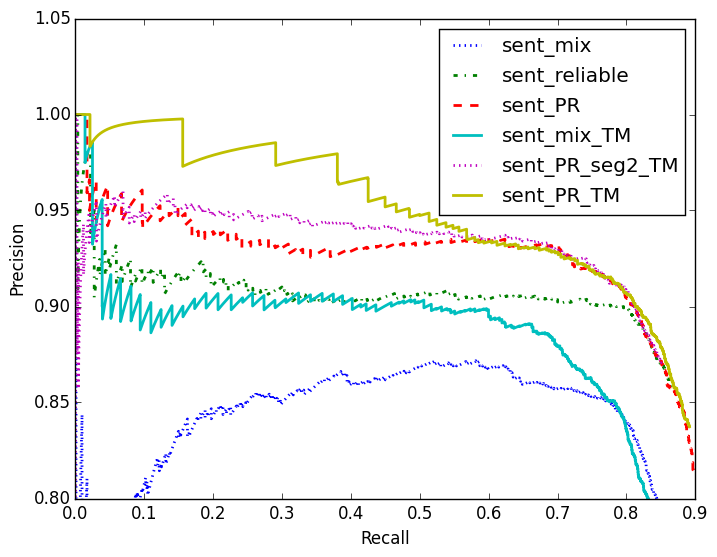
\includegraphics[width=0.9\linewidth]{figures/sent_time_exp_overall.png}
\caption{Sentence Level Results on TimeRE}
\label{fig: sent_luo}
\end{center}
\end{figure}

\subsection{Experimental Setup}

\paragraph{Hyperparameters} \red{can we put those parameters in a table?? especially those shared by the two settings.} \todo{ZW: Agree. These parameters should be given in a table!}
We experiment our sentence level model on \TimeRE. We use 100-dimensional word embedding pre-trained using GloVe \cite{pennington2014glove} on Wikipedia and Gigaword, and 20-dimensional vector for distance embedding. The convolution window is 3 and the number of convolution kernels is 200. The size of the full connection layer is also 200. As for training, we use stochastic gradient descend (SGD) with batch size 20, learning rate 0.1. We also use dropout with probability 0.5 upon the sentence embedding. Each data subset is added after 15 epochs since the precious one is added. The trace regularization parameters for three subsets are $\beta_1=-0.01$, $\beta_2=0.01$ and $\beta_3=0.1$ respectively from the reliable one to the most unreliable one (the ratio of $\beta_3$ and $\beta_2$ is fixed to 10 or 5 during hyper-parameter tuning).


The parameters of the bag level model is almost the same as the sentence level model on TimeRE data, except that the learning rate is 0.01. As for the \EntityRE data, the word embedding is of dimension 50 and is pre-trained on the NYT corpus using word2vec\footnote{\url{ https://code.google.com/p/word2vec/}}. The convolution window is 3 and the number of convolution kernels is 256, distance embedding size is 5, batch size is 16 and learning rate is 0.01. For all the bag level models, the linear combination parameter $\alpha$ is 1 and trace regularization parameter $\beta$ is -0.1 at the start of training. We experiment with decay rate \{0.95, 0.9, 0.8\} and decay step \{3, 5, 8\}. We find that using decay rate 0.9 and decay step 5 performs best in most situations.

\paragraph{Evaluation Metrics}
We evaluate the relation extraction performances using precision-recall (\PR) curves, which is calculated according to the extraction results ranked decreasingly by their confidence scores.

\paragraph{Baseline Settings}
We evaluate our approach under two extraction settings, sentence level
(\texttt{sent\_}) and bag level (\texttt{bag\_}). In both settings, we
investigate models trained on all subsets mixed together (\texttt{\_mix}),
models trained on reliable data only (\texttt{\_reliable}), models trained
with transition matrix (\texttt{\_TM}), and models trained
with the curriculum learning setting  (\texttt{\_CL}). In the bag level
experiments, we also study the effect of attention (\texttt{\_att}) and
average
(\texttt{\_avg}) aggregation methods.
\todo{ZW: This paragraph need to be polished.}

\begin{figure*}[htbp]
\centering
\subfigure[Attention Aggregation]{
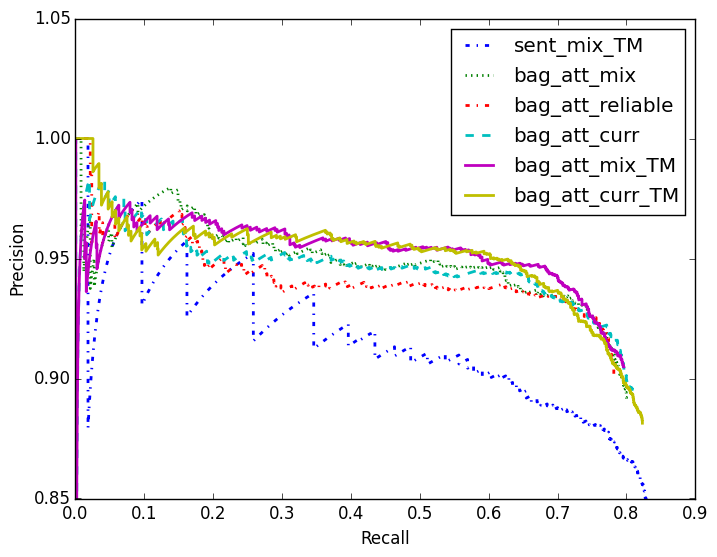
\includegraphics[width=0.45\linewidth]{figures/bag_att_exp_overall.png}
\label{fig: bag_att_luo}
}
\subfigure[Average Aggregation]{
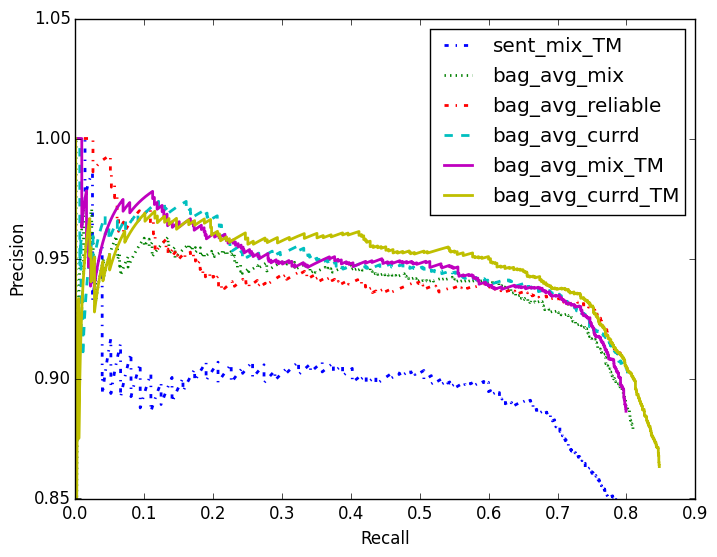
\includegraphics[width=0.45\linewidth]{figures/bag_avg_exp_overall.png}
\label{fig: bag_avg_luo}
}
\caption{Bag Level Results on TimeRE}
\label{fig: results_on_luo}
\end{figure*}

